% !TeX root = orbits.tex
% !TeX Program=pdfLaTeX

%%%%%%%%%%%%%%%%%%%%%%%%%%%%%%%%%%%%%%%%%%%%%%%%%%%%%%%%%%%%%%%%

\chapter{Gravitation}\label{s.newton}

In the \textit{Principia} Isaac Newton proved the following theorem.
\begin{quote}
\begin{theorem}
If a planet subject to a centripetal force follows an elliptical orbit around the Sun, then the force decreases as the inverse square of the distance from the Sun.
\end{theorem}
\end{quote}
After a review of Newton's Laws of force and motion,  we show that Kepler's second law must hold in \emph{any} system subject to a centripetal force. The next step is to show the inverse-square law and then it is a small step to universal gravitation and Kepler's third law.

\section{Newton's laws of motion and Kepler's second law}

%%%%%%%%%%%%%%%%%%%%%%%%%%%%%%%%%%%%%%%%%%%%%%%%%%%%%%%%%%%%%%%%

\begin{figure}[b]
\begin{minipage}{.45\textwidth}
\begin{center}
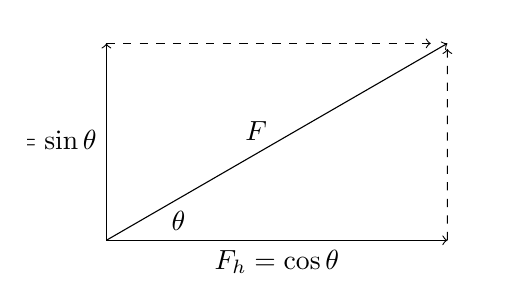
\begin{tikzpicture}
\clip (-1,-.5) rectangle +(6,3.2);
% Define center point
\coordinate (O) at (0,0);
\node[above right,xshift=20pt] at (O) {$\theta$};

% Construct force vector
\draw[->] (O) -- node[left,yshift=4pt] {$F$} +(30:5) coordinate (F);

% Construct horizontal component
\draw[->] (O) -- node[below] {$F_h=\cos \theta$} 
  +(0:4.33) coordinate (FH);
\draw[->,style={shorten >= 2pt},dashed] (FH) -- (F);

% Construct vertical component
\draw[->] (O) -- node[left] {$F_v=\sin \theta$} +(90:2.5) coordinate (FV);
\draw[->,style={shorten >= 6pt},dashed] (FV) -- (F);
\end{tikzpicture}
\caption{Perpendicular components\\of a force}\label{f.grav-forces1}
\end{center}
\end{minipage}
%%%%%%%%%%%%%%%%%%%%%%%%%%%%%%%%%%%%%%%%%%%%%%%%%%%%%%%%%%%%
\begin{minipage}{.45\textwidth}
\begin{center}
\begin{tikzpicture}
\clip (-1,-.5) rectangle +(6,3.2);
% Define center piont
\coordinate (O) at (0,0);

% Construct force vector
\draw[->] (O) -- node[left,yshift=4pt] {$F$} +(30:5) coordinate(F);

% Construct one component
\draw[->] (O) -- node[below,yshift=-2pt] {$F_1$} +(10:3) coordinate (F1);
\draw[->,style={shorten >= 4pt},dashed] (F1) -- (F);

% Construct other component
% First define end of component to allow shortened arrow
\path[dashed] (F) -- +(190:3) coordinate (F2);
\draw[->,style={shorten >= 6pt},dashed] (F2) -- (F);
\draw[->] (O) --  node[left,xshift=-3pt,yshift=2pt] {$F_2$} (F2);
\end{tikzpicture}
\caption{The parallelogram formed by two forces}\label{f.grav-forces2}
\end{center}
\end{minipage}
\end{figure}

%%%%%%%%%%%%%%%%%%%%%%%%%%%%%%%%%%%%%%%%%%%%%%%%%%%%%%%%%%%%

\begin{enumerate}
\item A body in uniform motion (including a body at rest) continues with the same motion unless a force is applied.
\item A force $F$ applied to a body causes an acceleration $a$ in the direction of the force whose magnitude is $a=F/m$, where $m$, the constant of proportionality, is the \emph{mass} of the body.
\item If one body exerts a force on a second body, the second body exerts a force on the first of equal magnitude but in the opposite direction.
\end{enumerate}
Forces are denoted by vectors, where the direction of the vector represents the direction of the force and the length of the vector represents the magnitude of the force. Forces can be decomposed into perpendicular components (Figure~\ref{f.grav-forces1}), or into components in any directions (Figure~\ref{f.grav-forces2}). The components form a parallelogram whose diagonal is the resultant force.

A \emph{centripetal force} is an attractive force exerted by a single body on another, in particular, the gravitational force exerted by the Sun on a planet (Figure~\ref{f.grav-centripetal}). Since this is the only force exerted on the planet, it does not move ``up'' or ``down'' and its orbit is in a plane.

%%%%%%%%%%%%%%%%%%%%%%%%%%%%%%%%%%%%%%%%%%%%%%%%%%%%%%%%%%%%%%%%

\begin{figure}[t]
\begin{minipage}{.48\textwidth}
\begin{center}
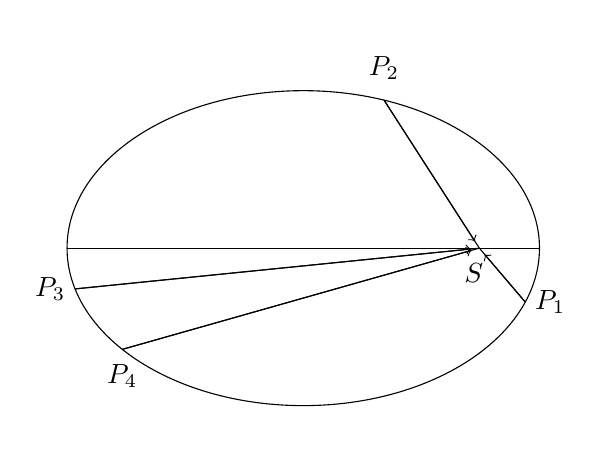
\begin{tikzpicture}
\clip (-3.5,-2.2) rectangle +(7,5);
% Size and center of the ellipse
\def\a{3}
\def\b{2}
\coordinate (O) at (0,0);

% Draw axis/axes through O
\coordinate (L) at (-180:{\a} and {\b});
\coordinate (R) at (0:{\a} and {\b});
\draw (L) -- (R);

% The Sun is at a focus
\coordinate (Sun) at ({+sqrt(\a*\a-\b*\b)},0);
\node[below,xshift=-2pt,yshift=-2pt] at (Sun) {$S$};

% Locate and label four arbitrary points on the list
\coordinate (P1) at +(-20:{\a} and {\b});
\draw (P1) node[right] {$P_1$} -- (Sun);
\coordinate (P2) at +(70:{\a} and {\b});
\draw (P2) node[above,yshift=4pt] {$P_2$} -- (Sun);
\coordinate (P3) at +(195:{\a} and {\b});
\draw (P3) node[left] {$P_3$} -- (Sun);
\coordinate (P4) at +(220:{\a} and {\b});
\draw (P4) node[below,yshift=-2pt] {$P_4$} -- (Sun);

% Draw the ellipse 
\draw (0,0) ellipse({\a} and {\b});

% Construct the arrows
\draw[->,style={shorten >= 3pt}] (P1) -- (Sun);
\draw[->,style={shorten >= 3pt}] (P2) -- (Sun);
\draw[->,style={shorten >= 3pt}] (P3) -- (Sun);
\draw[->,style={shorten >= 3pt}] (P4) -- (Sun);

\end{tikzpicture}
\caption{Centripetal force}\label{f.grav-centripetal}
\end{center}
\end{minipage}
%%%%%%%%%%%%%%%%%%%%%%%%%%%%%%%%%%%%%%%%%%%%%%%%%%%%%%%%%%%%
\begin{minipage}{.5\textwidth}
\begin{center}
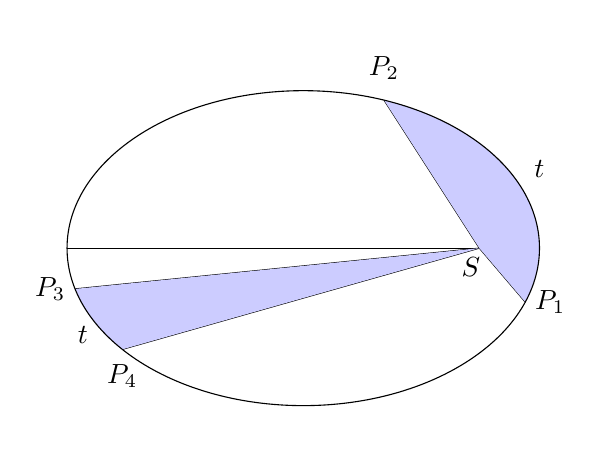
\begin{tikzpicture}
\clip (-3.5,-2.2) rectangle +(7,5);
% Size and center of the ellipse
\def\a{3}
\def\b{2}
\coordinate (O) at (0,0);

% Draw axis/axes through O
\coordinate (L) at (-180:{\a} and {\b});
\coordinate (R) at (0:{\a} and {\b});
\draw (L) -- (R);

% The Sun is at a focus
\coordinate (Sun) at ({+sqrt(\a*\a-\b*\b)},0);
\node[below,xshift=-3pt] at (Sun) {$S$};

% Locate and label four arbitrary points on the list
\coordinate (P1) at +(-20:{\a} and {\b});
\draw (P1) node[right] {$P_1$} -- (Sun);
\coordinate (P2) at +(70:{\a} and {\b});
\draw (P2) node[above,yshift=4pt] {$P_2$} -- (Sun);
\coordinate (P3) at +(195:{\a} and {\b});
\draw (P3) node[left] {$P_3$} -- (Sun);
\coordinate (P4) at +(220:{\a} and {\b});
\draw (P4) node[below,yshift=-2pt] {$P_4$} -- (Sun);

% Shade the sectors
\fill[blue!20] (Sun) -- (P1) arc [start angle = -20, end angle = 70,
    x radius = \a, y radius = \b] -- (P2) -- cycle;
\fill[blue!20] (Sun) -- (P3) arc [start angle = 195, end angle = 220,
    x radius = \a, y radius = \b] -- (P4) -- cycle;

% Draw the ellipse 
\draw (0,0) ellipse({\a} and {\b});

% Label the times and areas
\node at (3,1) {$t$};
\node at (-2.8,-1.1) {$t$};
\end{tikzpicture}
\caption{Equal areas in equal times}\label{f.grav-second}
\end{center}
\end{minipage}
\end{figure}

%%%%%%%%%%%%%%%%%%%%%%%%%%%%%%%%%%%%%%%%%%%%%%%%%%%%%%%%%%%%%%%%

Kepler's second law states that a planet in orbit sweeps out equal area in intervals of equal duration, that is, if it takes the planet time $t$ to move from $P_1$ to $P_2$ and also $t$ to move from $P_3$ to $P_4$, then the area of the sector $P_1SP_2$ is equal to the area of $P_3SP_4$ (Figure~\ref{f.grav-second}). It follows that the speed of the planet must vary as it traverses its orbit ($v_{P_1P_2} \gg v_{P_3P_4}$). Kepler's second law holds for any two-body system subject to a centripetal force; the force need not be inverse-square.

%%%%%%%%%%%%%%%%%%%%%%%%%%%%%%%%%%%%%%%%%%%%%%%%%%%%%%%%%%%%

\begin{figure}[b]
\begin{minipage}{.48\textwidth}
\begin{center}
\begin{tikzpicture}[scale=1.4]
\clip (2,-.4) rectangle +(3.3,4.5);

% Size and center of the ellipse
\def\a{5.25}
\def\b{3.5}
\coordinate (O) at (0,0);

% The Sun is at a focus
\coordinate (S) at (2.5,0);
\node[below] at (S) {$S$};

% Construct the ellipse
\draw[name path=ellipse] (5,0) arc(0:60:5cm and 4cm);

% Locate and label three arbitrary points on the list
\path [name path=a] (S) -- ($(S)+(10:4)$);
\path [name intersections = {of = ellipse and a, by = {A} }];
\draw (S) -- (A) node[right] {$A$};
\path [name path=b] (S) -- ($(S)+(50:4)$);
\path [name intersections = {of = ellipse and b, by = {B} }];
\draw (S) -- (B) node[above right] {$B$};
\path [name path=c] (S) -- ($(S)+(82:4)$);
\path [name intersections = {of = ellipse and c, by = {C} }];
\draw (S) -- (C) node[above right] {$C$};

% Label A, B, C
\path (A) --
  node[right,xshift=6pt,yshift=2pt] {$\Delta t$} (B) -- 
  node[above right,xshift=2pt] {$\Delta t$} (C);

\end{tikzpicture}
\caption{``Small'' sectors of an orbit}\label{f.grav-very-small}
\end{center}
\end{minipage}
%%%%%%%%%%%%%%%%%%%%%%%%%%%%%%%%%%%%%%%%%%%%%%%%%%%%%%%%%%%%
\begin{minipage}{.48\textwidth}
\begin{center}
\begin{tikzpicture}[scale=1.4]
\clip (2,-.4) rectangle +(3.3,4.5);

% Size and center of the ellipse
\def\a{5.25}
\def\b{3.5}
\coordinate (O) at (0,0);

% The Sun is at a focus
\coordinate (S) at (2.5,0);
\node[below] at (S) {$S$};

% Construct the ellipse
\draw[name path=ellipse] (5,0) arc(0:60:5cm and 4cm);

% Locate and label three arbitrary points on the list
\path [name path=a] (S) -- ($(S)+(10:4)$);
\path [name intersections = {of = ellipse and a, by = {A} }];
\draw (S) -- (A) node[right] {$A$};
\path [name path=b] (S) -- ($(S)+(50:4)$);
\path [name intersections = {of = ellipse and b, by = {B} }];
\draw (S) -- (B) node[above right] {$B$};

% Label A, B, C
\path (A) --
  node[right,xshift=6pt,yshift=2pt] {$\Delta t$} (B) -- (C);

% Draw AB
\draw (A) -- (B) -- (C);

% Locate C' twice the length AB from A
\path (A) -- ($(A) ! 2 ! (B)$) coordinate (CP);
\vertexsm{CP};
\draw[thick,dashed] (B) -- 
  node[above right] {$\Delta t$} (CP) node[above left] {$C'$};

% Draw vector in the direction of BS
%  and locate its intersection with the ellipse
% Locate Cnew as the correct location of C
\path[name path=cp] (CP) -- +(230:2);
\path [name intersections = {of = cp and ellipse, by = {Cnew} }];
\draw[very thick,dashed,->] (CP) -- 
  (Cnew) node[above,xshift=-2pt,yshift=4pt] {$C$};
\draw (Cnew) -- (S);

% Draw the force arrow
\path (CP) -- ($(CP)!1.5!(Cnew)$) coordinate (CX) --
  ($(CP)!2.5!(Cnew)$) coordinate (CY);
\draw[->,thick] (CX) -- node[left,near start,xshift=-2pt] {$F_B$} (CY);

\path[->,thick] ($(B)+(-4pt,0)$) coordinate (B1) -- 
  ($(S)+(-4pt,0)$) coordinate (S1);
\draw[->,thick] ($(B1)!.15!(S1)$) -- 
  node[left,near start] {$F_P$} ($(B1)!.43!(S1)$);

\end{tikzpicture}
\caption{Exerting force at discrete times}\label{f.grav-small}
\end{center}
\end{minipage}
\end{figure}

%%%%%%%%%%%%%%%%%%%%%%%%%%%%%%%%%%%%%%%%%%%%%%%%%%%%%%%%%%%%

The proof is based on dividing an area into very small sectors and then taking the limit. Consider three points $A,B,C$ on the orbit (Figure~\ref{f.grav-very-small}) that represent the positions of the planet at intervals of $\Delta t$. For clarity we have drawn them spaced out, but the intention is that they are very close together. Newton assumed that the planet does not smoothly traverse the arcs, but rather that it every $\Delta t$ it jumps in discrete steps from one point on the orbit to the next.

Figure~\ref{f.grav-small} shows how the force is exerted in discrete steps. The planet moves from $A$ to $B$ and we expect that the centripetal force at $B$ will cause an acceleration that moves the planet to $C$, the next point on the orbit. Instead, we ``pretend'' that the force is not applied at $B$, but, in the absence of an applied force, planet continues with the same velocity. After another period of $\Delta t$ as passed and the planet has reached point $C'$, the force is now applied \emph{in the same direction} as it would have been applied at $B$, moving the planet to $C$. 

\begin{theorem}
The area of $\triangle ASB$ is equal to the area of $\triangle BSC$.
\end{theorem}

%%%%%%%%%%%%%%%%%%%%%%%%%%%%%%%%%%%%%%%%%%%%%%%%%%%%%%%%%%%%%%%%

\begin{figure}[t]
\begin{minipage}{.48\textwidth}
\begin{center}
\begin{tikzpicture}[scale=1.4]
\clip (2,-.4) rectangle +(3.5,4.5);

% Size and center of the ellipse
\def\a{5.25}
\def\b{3.5}
\coordinate (O) at (0,0);

% The Sun is at a focus
\coordinate (S) at (2.5,0);
\node[below] at (S) {$S$};

% Construct the ellipse
\draw[name path=ellipse] (5,0) arc(0:60:5cm and 4cm);

% Locate and label three arbitrary points on the list
\path [name path=a] (S) -- ($(S)+(10:4)$);
\path [name intersections = {of = ellipse and a, by = {A} }];
\draw (S) -- (A) node[right] {$A$};
\path [name path=b] (S) -- ($(S)+(50:4)$);
\path [name intersections = {of = ellipse and b, by = {B} }];

% Draw triangle SAB
\draw[blue] (S) -- (A) -- (B);
\draw[blue] ($(S)+(2pt,0)$) -- ($(B)+(2pt,0)$);

% Locate C' twice the length AB from A
\path (A) -- ($(A) ! 2 ! (B)$) coordinate (CP);
\node[above] at (CP) {$C'$};

% Draw vector in the direction of BS
%  and locate its intersection with the ellipse
% Locate Cnew as the correct location of C
\path[name path=cp] (CP) -- +(230:2);
\path [name intersections = {of = cp and ellipse, by = {Cnew} }];
\draw[red] (B) -- (CP) -- (S) -- cycle;
\node[above,xshift=-2pt,yshift=2pt] at (Cnew) {$C$};
\draw (S) -- (Cnew);
\vertexsm{CP};

% Draw altitude to ABC'
\coordinate (H) at ($(A)!(S)!(CP)$);
\node[right,xshift=6pt,yshift=2pt] at (H) {$H$};
\draw[thick,dashed,red] (H) -- (S);
\draw[thick,dashed,blue] ($(H)+(1pt,-1pt)$) -- ($(S)+(1pt,-1pt)$);
\draw[rotate=115] (H) rectangle +(4pt,4pt);

\draw (S) -- (B) node[above right] {$B$} -- (C);

\end{tikzpicture}
\caption{$\triangle ASB=\triangle BSC'$}\label{f.grav-areas1}
\end{center}
\end{minipage}
%%%%%%%%%%%%%%%%%%%%%%%%%%%%%%%%%%%%%%%%%%%%%%%%%%%%%%%%%%%%%%%%%%%%%%%
\begin{minipage}{.48\textwidth}
\begin{center}
\begin{tikzpicture}[scale=1.4]
\clip (1.8,-.4) rectangle +(3.7,4.5);

% Size and center of the ellipse
\def\a{5.25}
\def\b{3.5}
\coordinate (O) at (0,0);

% The Sun is at a focus
\coordinate (S) at (2.5,0);
\node[below] at (S) {$S$};

% Construct the ellipse
\draw[name path=ellipse] (5,0) arc(0:60:5cm and 4cm);

% Locate and label three arbitrary points on the list
\path [name path=a] (S) -- ($(S)+(10:4)$);
\path [name intersections = {of = ellipse and a, by = {A} }];
\draw (S) -- (A) node[right] {$A$};
\path [name path=b] (S) -- ($(S)+(50:4)$);
\path [name intersections = {of = ellipse and b, by = {B} }];
\draw (A) -- (B) node[below,xshift=-2pt,yshift=-4pt] {$B$};

% Locate C' twice the length AB from A
\path (A) -- ($(A) ! 2 ! (B)$) coordinate (CP);
\node[above] at (CP) {$C'$};

% Draw vector in the direction of BS
%  and locate its intersection with the ellipse
% Locate Cnew as the correct location of C
\path[name path=cp] (CP) -- +(230:2);
\path [name intersections = {of = cp and ellipse, by = {Cnew} }];
\draw[red] (B) -- (CP) -- (S) -- cycle;
\node[above,xshift=-2pt,yshift=2pt] at (Cnew) {$C$};
\draw (S) -- (Cnew);
\vertexsm{CP};
\draw[blue] ($(S)-(2pt,0)$) -- ($(B)+(-1pt,1pt)$) coordinate (rect1) -- node[black,below] {$h$}  (Cnew) -- (S);
\draw[rotate=140] (rect1) rectangle +(4pt,4pt);

% Draw parallels CC', SB
\draw[thick,dashed] ($(Cnew)!-2cm!(CP)$) -- ($(Cnew)!1.3cm!(CP)$);
\draw[thick,dashed] (B) -- ($(S)!4.3cm!(B)$);

% Draw height between parallels
\draw[red,dashed,thick] (CP) -- ($(S)!(CP)!(B)$) coordinate (rect2);
\draw[rotate=140] (rect2) rectangle +(4pt,4pt);

\end{tikzpicture}
\caption{$\triangle BSC'=\triangle BSC$}\label{f.grav-areas2}
\end{center}
\end{minipage}
\end{figure}

%%%%%%%%%%%%%%%%%%%%%%%%%%%%%%%%%%%%%%%%%%%%%%%%%%%%%%%%%%%%%%%%

\begin{proof}
The proof will be done in two steps by showing that $\triangle ASB=\triangle BSC'$ and then that $\triangle BSC'=\triangle BSC$.
\begin{itemize}
\item In Figure~\ref{f.grav-areas1}, $\triangle ASB$ is shown in blue and $\triangle BSC'$ is shown in red. It is assumed that $AB=BC'$ (the planet moves from $B$ to $C'$ during the same interval $\Delta t$), so since $SH$ is the height of both triangles, their areas are equal.
\item In Figure~\ref{f.grav-areas2}, $\triangle BSC$ is shown in blue and $\triangle BSC'$ is shown in red. It is assumed $CC'$ is parallel to $SB$ (the planet is subject to the centripetal force at $C'$ in the \emph{same} direction as the force at $B$), so the heights of both triangles to the common side $SB$ are equal and their areas are equal. It follows that $\triangle BSC'=\triangle BSC=\triangle ASB$.\hqed
\end{itemize}
\end{proof}

We assume that the sectors of the orbit are each divided up into small sectors of uniform duration $\Delta t$. By the theorem, each sector has the same area $\Delta A$. Therefore (see Figure~\ref{f.grav-second}),
\[
\frac{A_{P_1SP_2}}{\Delta A} =\frac{t}{\Delta t} = \frac{A_{P_3SP_4}}{\Delta A}\,,
\]
from which Kepler's second law follows: $A_{P_1SP_2}=A_{P_3SP_4}$.

The proof used two approximations:
\begin{itemize}
\item $\Delta A$ is an approximation of the area of each sector.
\item The force at $C'$ is an approximation to the force at $B$.
\end{itemize}
In the limit as the size of the sectors decreases, the errors become negligible.

\begin{definition}\label{def.kappa}
For a given elliptical orbit, $\kappa=A/t$, where $A$ is the area of the ellipse and $t$ is the period of the orbit, is called \emph{Kepler's constant}.
\end{definition}

%%%%%%%%%%%%%%%%%%%%%%%%%%%%%%%%%%%%%%%%%%%%%%%%%%%%%%%%%%%%

\section{The inverse square law for gravitation}

Newton's next step was to show that if the orbit of a planet is elliptical, the centripetal force must be proportional to the mass of the planet and inversely proportional to the square of its distance from the Sun. In Figure~\ref{f.grav-inverse1}, $S$ is the Sun, and $P$ and $Q$ are points on the orbit that are very close to each other. $PR$ is the tangent to the ellipse at $P$, and $R$ is chosen to that $QR$ is parallel to $SP$.  $QT$ is constructed perpendicular to $SP$. Denote the lengths $r_P=SP$, $h=QT$, $q=QR$ and the time interval from $P$ to $Q$ by $\Delta t$.

%%%%%%%%%%%%%%%%%%%%%%%%%%%%%%%%%%%%%%%%%%%%%%%%%%%%%%%%%%%%

\begin{figure}[t]
\begin{center}
\begin{tikzpicture}

\clip (-4.6,-.6) rectangle +(9.5,4.3);

% Size and center of the ellipse
\def\a{4.5}
\def\b{3}
\def\angle{10}

\pic{semi-ellipse={\a}/{\b}};
\pic{point-on-ellipse={\a}/{\b}/{\angle}};
\pic{tangent={\a}/{\b}/{\angle}};
\node[below] at (F1) {$S$};
\draw (F1) -- node[above] {$r_p$} (P);

% Select an arbitrary point Q on the ellipse and draw a line to the Sun
\path[name path=fromF1q] (F1) -- +(20:8);
\path [name intersections = {of = ellipse and fromF1q, by = {Q} }];
\draw (F1) -- (Q);
\node[above] at (Q) {$Q$};

% Draw PQ
\draw[thick,dashed] (P) -- (Q);

% Draw QR
\path[name path=qr] (Q) -- +(7:2);
\path [name intersections = {of = t and qr, by = {R} }];
%\vertexsm{R};
\node[above right] at (R) {$R$};
\draw (Q) -- node[above] {$q$} (R);

% Draw QX
\path[name path=qx] (Q) -- +({\angle-90}:{1.5*\a} and {1.5*\b});
\path [name intersections = {of = qx and fromF1p, by = {X} }];
\draw (Q) -- (X);

% Draw the force arrows
\coordinate (PX) at ($(P)+(0,5pt)$);
\coordinate (SX) at ($(F1)+(0,5pt)$);
\draw[->,thick] ($(PX)!.27!(SX)$) -- 
  node[above] {$F_P$} ($(PX)!.43!(SX)$);

% Draw force arrow from Q
\path (R) -- ($(R)!1.7!(Q)$) coordinate (RX) --
  ($(R)!3!(Q)$) coordinate (RY);
\draw[->,thick] (RX) -- node[above] {$F_P$} (RY);

% Draw force arrow from P
\draw (Q) -- node[left] {$h$} ($(F1)!(Q)!(P)$) coordinate (T);
\node[below] at (T) {$T$};
\draw[rotate=96] (T) rectangle +(6pt,6pt);

\end{tikzpicture}
\caption{The derivation of the inverse square law}\label{f.grav-inverse1}
\end{center}
\end{figure}

When a point is subject to an acceleration $a$ for a period of $\Delta t$, its displacement is $\frac{1}{2} a (\Delta t)^2$. From Newton's second law we know that at point $R$, the planet is subjected to an acceleration of $F_P/m$, so
\begin{eqn}
q &=& \frac{1}{2}\frac{F_P}{m} (\Delta t)^2\\[4pt]
F_P &=& \frac{2mq}{(\Delta t)^2}\,.
\end{eqn}%

Now we compute the area of the sector $PSQ$ which is approximately the area of $\triangle SPQ = (1/2)hr_p$ and use Kepler's constant:
\begin{eqn}
\Delta t &=& \frac{\Delta A_{PSQ}}{\kappa}=\frac{hr_P}{2\kappa}\\[2pt]
F_P &=& 2mq\cdot\frac{4\kappa^2}{(hr_P)^2}= 8\kappa^2m\cdot\frac{q}{h^2}\cdot \frac{1}{r_P^2}\,.
\end{eqn}%
To obtain an inverse-square law for the force, the first two factors have to be independent of the distance. For a given planet $m$ is constant and for a given elliptical orbit $\kappa$ is constant, so the first factor does not depend on the distance. What about the second factor $q/h^2$, in particular, what value does it have as $\Delta t$ approaches zero?
\begin{theorem}\label{thm.lr-limit}
In an elliptical orbit
\[
\lim_{\Delta t \rightarrow 0} \frac{q}{h^2} = \frac{1}{L}\,,
\]
where $L$ is the length of the latus rectum of the ellipse (Definition~\ref{def.ellipse-lr}).
\end{theorem}
Newton's proof is very complex and is presented separately in Chapter~\ref{s.centripetal}.

Since $L$ is constant for any given ellipse, the inverse square law can be written
\begin{equation}
F_P = \frac{8\kappa^2m}{L}\cdot\frac{1}{r_P^2}\,.\label{eqn.inverse}
\end{equation}%
The formula can be re-written so that the constant values appearing are more familiar: $a$, the semi-major axis and $T$, the period of the orbit. By Theorem~\ref{thm.ellipse-lr}, $L\!\!=\!\!2b^2/a$ and by Theorem~\ref{thm.ellipse-area}, $A_e$, the area of the ellipse is $\pi a b$. Therefore, $\kappa = A_e/T\!\!=\!\!\pi ab/T$ and
\begin{equation}
F_P = \frac{8\kappa^2 m}{L}\cdot\frac{1}{r_P^2}
=\frac{8(\pi a b)^2 m}{T^2}\cdot \frac{a}{2b^2}\cdot\frac{1}{r_P^2}
=\frac{4\pi^2 a^3 m}{T^2}\cdot\frac{1}{r_P^2}\,.\label{eqn.planet-force}
%F_P = \frac{8\kappa^2 am}{2b^2}\cdot\frac{1}{r_P^2}
%=\frac{4\pi^2 a^2 b^2 am}{b^2 T^2}\cdot \frac{1}{r_P^2}
%=\frac{4\pi^2 a^3 m}{T^2}\cdot\frac{1}{r_P^2}\,.\label{eqn.planet-force}
\end{equation}%
Newton was able to show that:
\begin{itemize}
\item The inverse square law applies to all conic sections including parabolas and hyperbolas and, of course, a circle which is a special case of an ellipse.
\item The converse holds: if a planet is subject to an inverse-square centripetal force then the orbit must be an ellipse (or another conic section).
\item The proof assumes that a planet is a very small point, but the result holds even for large planets as long as the density of the planet is radially symmetric, that is, for a given distance from the center the density is constant.
\end{itemize}

%%%%%%%%%%%%%%%%%%%%%%%%%%%%%%%%%%%%%%%%%%%%%%%%

\section{Universal gravitation}

By Newton's third law, we can equate the force $F_{S\leftarrow E}$ that the Sun $S$ exerts on the Earth $E$ with the force $F_{E\leftarrow S}$ that the Earth exerts on the Sun. Let $m$ be the mass of the Earth and $M$ be the mass of the Sun, then by Equation~\ref{eqn.inverse},
\begin{eqn}
F_{S\leftarrow E} &=& \frac{8\kappa_E^2m}{L_E}\cdot\frac{1}{r^2}=\frac{C_Em}{r^2}\\[4pt]
F_{E\leftarrow S} &=& \frac{8\kappa_S^2M}{L_S}\cdot\frac{1}{r^2}=\frac{C_SM}{r^2}\\[4pt]
\frac{C_E}{M}\cdot\frac{1}{r^2}&=&\frac{C_S}{m}\cdot\frac{1}{r^2}\,,
\end{eqn}%
from some constants $C_E,C_S$.

Why are the constants different? The Earth and the Sun both rotate around their center of mass called the \emph{barycenter}, which is very close to the center of the Sun since the Sun is so much more massive than the Earth. The ellipse of the Sun's orbit is very small relative to the Earth so $A$ and $L$ are smaller, and the Sun's period is large so $T$ is larger. The different values for $8\kappa^2/L$ are encapsulated into the constants $C_E,C_S$. Let $G=\displaystyle\frac{C_E}{M}=\frac{C_S}{m}$ so that
\begin{equation}
F_{S\leftarrow E}=F_{E\leftarrow S}=G\frac{mM}{r^2}\,.\label{eqn.universal}
\end{equation}%
This is Newton's law of universal gravitation. It is not specific to planetary orbits but holds between any two bodies with masses $m,M$.

\section{Kepler's third law}

\begin{theorem}[Kepler's third law]
Let $P_1, P_2$ be two planets whose elliptical orbits have semi-major axes $a_1, a_2$ and whose orbital periods around the Sun are $T_1$ and $T_2$. Then
\[
\frac{a_1^3}{T_1^2}=\frac{a_2^3}{T_2^2}\,.
\]
\end{theorem}
\begin{proof}
By Equations~\ref{eqn.planet-force} and~\ref{eqn.universal},
\begin{equation}
F=\frac{4\pi^2 a_i^3 m}{T_i^2}\frac{1}{r_i^2}=\frac{GmM}{r_i^2}\,.\label{eqn.third-law}
\end{equation}
After canceling $m$ and $r_i$ we get
\[
\frac{a_i^3}{T_i^2}=\frac{GM}{4\pi^2}\,.
\]
$GM/4\pi^2$ is a constant that depends only on the mass of the Sun and the gravitational constant, so $a_i^3/T_i^2$ is constant for all planets rotating around the Sun.\hqed
\end{proof}
